This chapter introduces the key aspects of the CERN Large Hadron Collider (LHC) and the Compact Muon Solenoid (CMS) experiment where the work for this thesis was conducted. Section \ref{section:LHC} describes the history of accelerator developments at CERN that led to the construction of the LHC, the current LHC configuration, and the largest experiments located at the LHC. The concepts of beam luminosity and pileup, which are critical for understanding and measuring high-energy particle collisions, are described in Section \ref{section:luminosity_and_pileup} and discussed in the context of the High-Luminosity LHC (HL-LHC) upgrade in Section \ref{section:HL-LHC}. Lastly, Section \ref{section:cms-detector} describes the design and function of CMS and its subdetectors, and terminates in a description of data processing at CMS, beginning from online event filtering in the Level-1 Trigger, to processing in the High-Level Trigger, to offline particle reconstruction, and finally long-term storage and processing of measured events.

\section{The Large Hadron Collider}
\label{section:LHC}
CERN, the European Organization for Nuclear Research, is an international organization based in Meyrin, Switzerland which operates the world's largest particle physics laboratory, and is the site of the Large Hadron Collider (LHC)~\cite{history_of_CERN}. The very first accelerator built at CERN was the 600\MeV Synchrocyclotron (SC), which initially provided beams for CERN's first experiments. The newer and more powerful Proton Synchrotron (PS), which could accelerate particles to an energy of 28\GeV, began operations in 1959 and is still in use today. The first hadron collider at CERN was the Intersecting Storage Rings (ISR), which consisted of two interlaced rings each with a diameter of 200. The ISR collided protons at a center-of-mass energy of 62\GeV and began measuring collisions in 1971. In 1968 CERN began to accelerate heavy ions in the Super Proton Synchrotron (SPS), which is 7 kilometers in circumference and was the first of CERN's giant underground rings to be built. The SPS became the forefront of CERN's particle physics program in 1976, and in 1981 was converted into a proton-antiproton collider. The final and largest underground ring constructed at CERN was the Large Electron-Positron (LEP) collider, which was commissioned in July 1989 and hosted 5176 magnets and 128 accelerating cavities located around a 27-kilometer circumference. Over 11 years of research, four detectors, ALEPH, DELPHI, L3, and OPAL measured the collisions, with collision energies reaching up to 209\GeV in the year 2000. In November 2000, LEP was closed down to make way for the construction of the LHC in the same tunnel.

In its current configuration, the LHC accelerator complex at CERN is a succession of machines that accelerate particles in stages until they reach their final energy of 6.5\TeV per beam~\cite{CERN-OPEN-2000-148}~\cite{Linac4-design-report-2020}. In Linear accelerator 4 (Linac4), negative hydrogen ions (hydrogen atoms with an additional electron) are accelerated to 160\MeV, and stripped of their two electrons, leaving only protons, before entering the Proton Synchrotron Booster (PSB). These protons are accelerated to 2\GeV, then to 26\GeV in the Proton Synchrotron (PS), and 450\GeV in the Super Proton Synchrotron (SPS). The protons are transferred to the two beam pipes of the Large Hadron Collider (LHC). The LHC is a 27-kilometer ring of superconducting magnets, inside which one beam circulates clockwise and the other counterclockwise. Each LHC ring takes 4 minutes and 20 seconds to fill, and it takes about 20 minutes for the protons to reach their maximum energy. During normal operating conditions, beams circulate for many hours inside the LHC ring. 

The beams of particles in the LHC are made to collide at a center-of-mass energy of up to 14\TeV, at four positions at particle detector experiments located around the ring: ATLAS, CMS, ALICE, and LHCb. An aerial view of the four major experiments' locations is shown in Fig. \ref{fig:aerial-view-LHC-ring}~\cite{OPEN-PHO-ACCEL-2017-005}. ATLAS and CMS are the two general-purpose detectors with broad physics programmes spanning Standard Model measurements and searches for signatures of new physics~\cite{ATLAS-TDR-14}~\cite{CERN-LHCC-2006-001}. The two experiments use different technical solutions and different magnet system designs. ALICE is a general-purpose detector dedicated to measuring LHC heavy-ion collisions, and is designed to address the physics of strongly interacting matter, and the properties of quark-gluon plasma~\cite{ALICE-original-TDR}. The LHCb experiment specializes in investigating CP violation through measuring the differences in matter and antimatter, by using a series of subdetectors to detect mainly forward particles close to the beam direction~\cite{LHCb-1998}. 

\begin{figure}[ht]
    \centering
    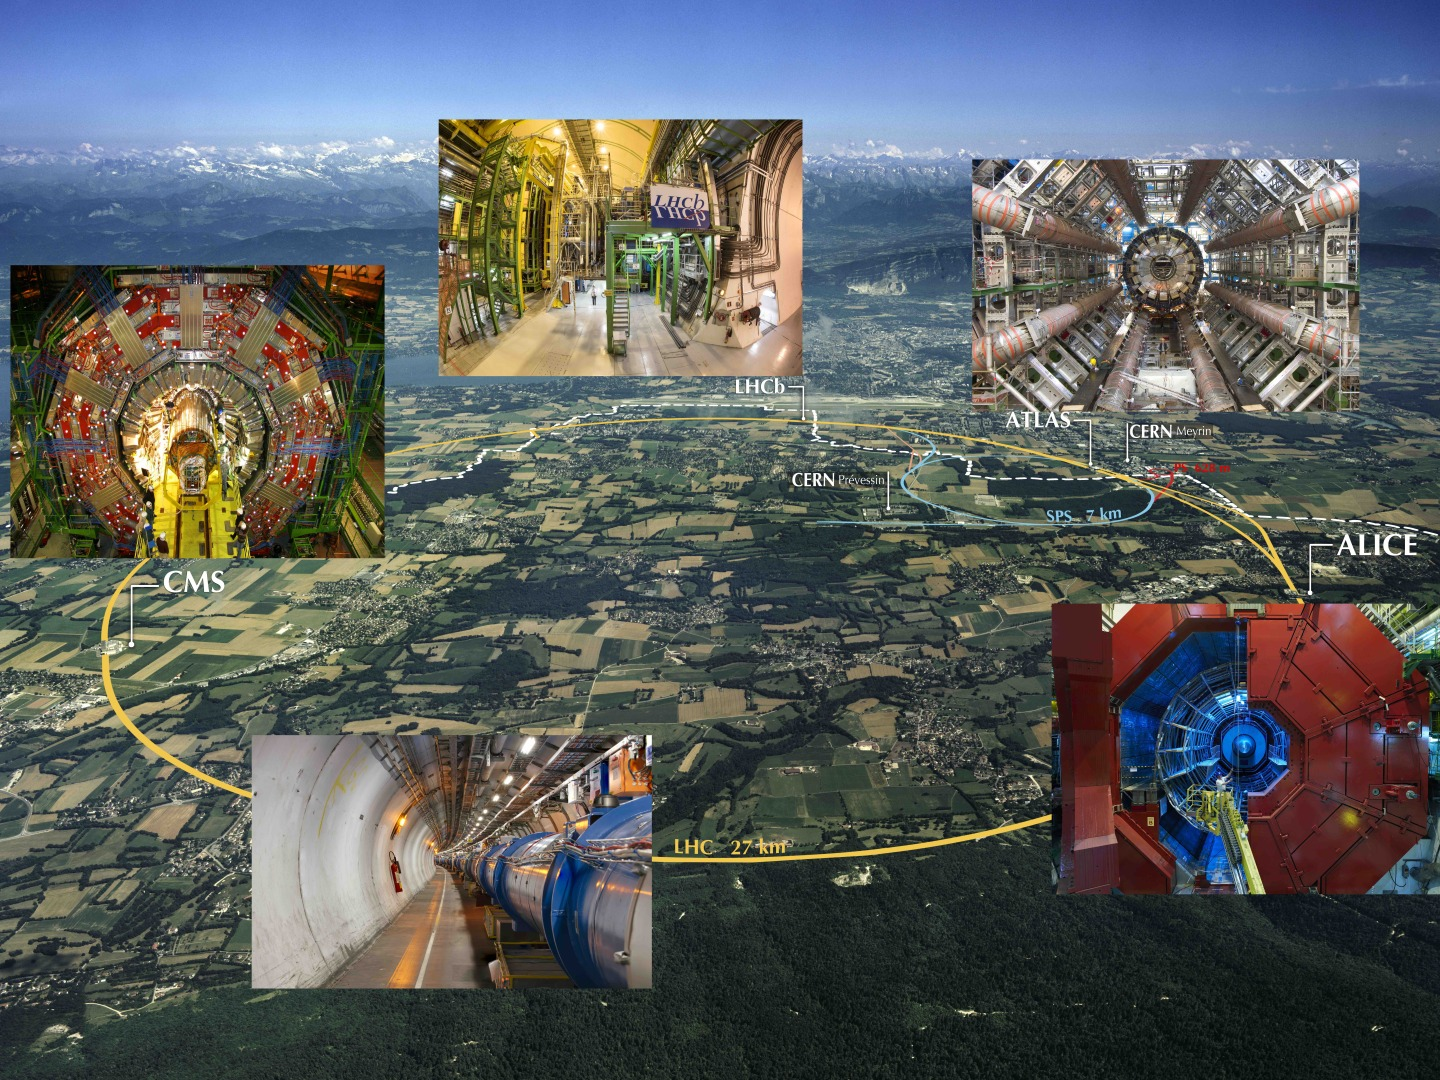
\includegraphics[width=11cm]{figures/ch-2-cern-cms/aerial-view-LHC-ring.jpeg}
    \caption[Aerial view of the Large Hadron Collider (LHC).]{Aerial view of the Large Hadron Collider (LHC) spanning the border of France and Switzerland, and the four major experiments located around the ring: CMS (Compact Muon Solenoid), LHCb (LHC beauty), ATLAS (A Toroidal LHC Apparatus), and ALICE (A Large Ion Collider Experiment)~\cite{OPEN-PHO-ACCEL-2017-005}.}
    \label{fig:aerial-view-LHC-ring}
\end{figure}



\section{Luminosity and pileup}
\label{section:luminosity_and_pileup}
In order to search for rare processes, such as those resulting from a Higgs, W, or Z boson, a large number of parton interactions per second are required at the LHC. The number of events generated per second by the LHC collisions is given by
\begin{equation}
     N_{event} = \mathcal{L} \cdot \sigma_{event}
    \label{eqn:nEvents}
\end{equation} 
where $\sigma_{event}$ is the cross-section for the event under study, and $\mathcal{L}$ the instantaneous luminosity. The instantaneous luminosity is measured in units of cm$^{-2}$ s$^{-1}$, and depends only on the beam parameters, and can be written for a Gaussian beam distribution as:
\begin{equation}
    \mathcal{L} = \frac{N_b^2 n_b f_{rev} \gamma_r}{4\pi \epsilon_n \beta^*} F
\end{equation}
where the parameters are as defined, along with some example typical nominal values in Phase-1 of the LHC~\cite{CERN-luminosity-accelerator-school-article}~\cite{ipac2012-proceedings}:
% reference: material included in introduction to accelerator physics 2021 https://indico.cern.ch/event/1001431/contributions/

\begin{itemize}
    \item $N_b$ is the number of particles per bunch ($N_b \approx 1.15 \times 10^{11}$ protons per bunch)
    \item $n_b$ is the number of bunches per beam (maximum 2808),
    \item $f_{rev}$ is the revolution frequency ($\approx 11$ kHz),
    \item $\gamma_r$ is the relativistic gamma factor,
    \item $\epsilon_n$ is the normalized transverse beam emittance (area in a transverse plane occupied by the beam particles),
    \item $\beta^*$ is the beta function at the collision point ($\beta^* = 0.55$ m),
    \item and $F$ is the geometric luminosity reduction factor due to the crossing angle at the interaction points ($F \approx 0.84$ for Phase-1. Note that complete overlap would give $F = 1$).
\end{itemize}
Peak luminosity at interaction points 1 and 5 reach values of $\sim 1.0 \times 10^{34}$ cm$^{-2}$ s$^{-1}$, with peak luminosity per bunch crossing reaching $\sim 3.56 \times 10^{34}$ cm$^{-2}$ s$^{-1}$.

Per Eqn. \ref{eqn:nEvents}, the integrated luminosity over time is proportional to the number of events produced, and the size of LHC datasets is commonly presented in terms of integrated luminosity. Collider operation aims to optimize the integrated luminosity. Thus the exploration of rare events in the LHC collisions requires both high beam energies and high beam intensities.

The interaction vertex corresponding to the hard scattering of the protons is called the primary interaction vertex, or primary vertex (PV). The LHC's nominal beam luminosities are sufficiently large for multiple proton-proton collisions to occur in the same time window of 25 nanoseconds in which proton bunches collide~\cite{CMS-JME-18-001}. To measure a proton-proton collision, the primary vertices must be separated from overlapping collisions, called ``pileup'' collisions. 

The pileup is defined as the average number of $pp$ collisions per bunch crossing, and can be estimated from the inelastic $pp$ cross section of $\sigma_{\text{inel}} = 68.6$ millibarns at a center-of-mass energy of $\sqrt{s} = 13$\TeV~\cite{CERN-EP-2018-004-pileup}:
\begin{equation}
    \text{Pileup} = \frac{\mathcal{L} \times \sigma_{\text{inel}}}{ n_b \cdot f} \sim 22
\end{equation}
A distribution of pileup in the data-taking years 2016-2018 is shown in Fig. \ref{fig:pileup-run-2}.

\begin{figure}[ht]
    \centering
    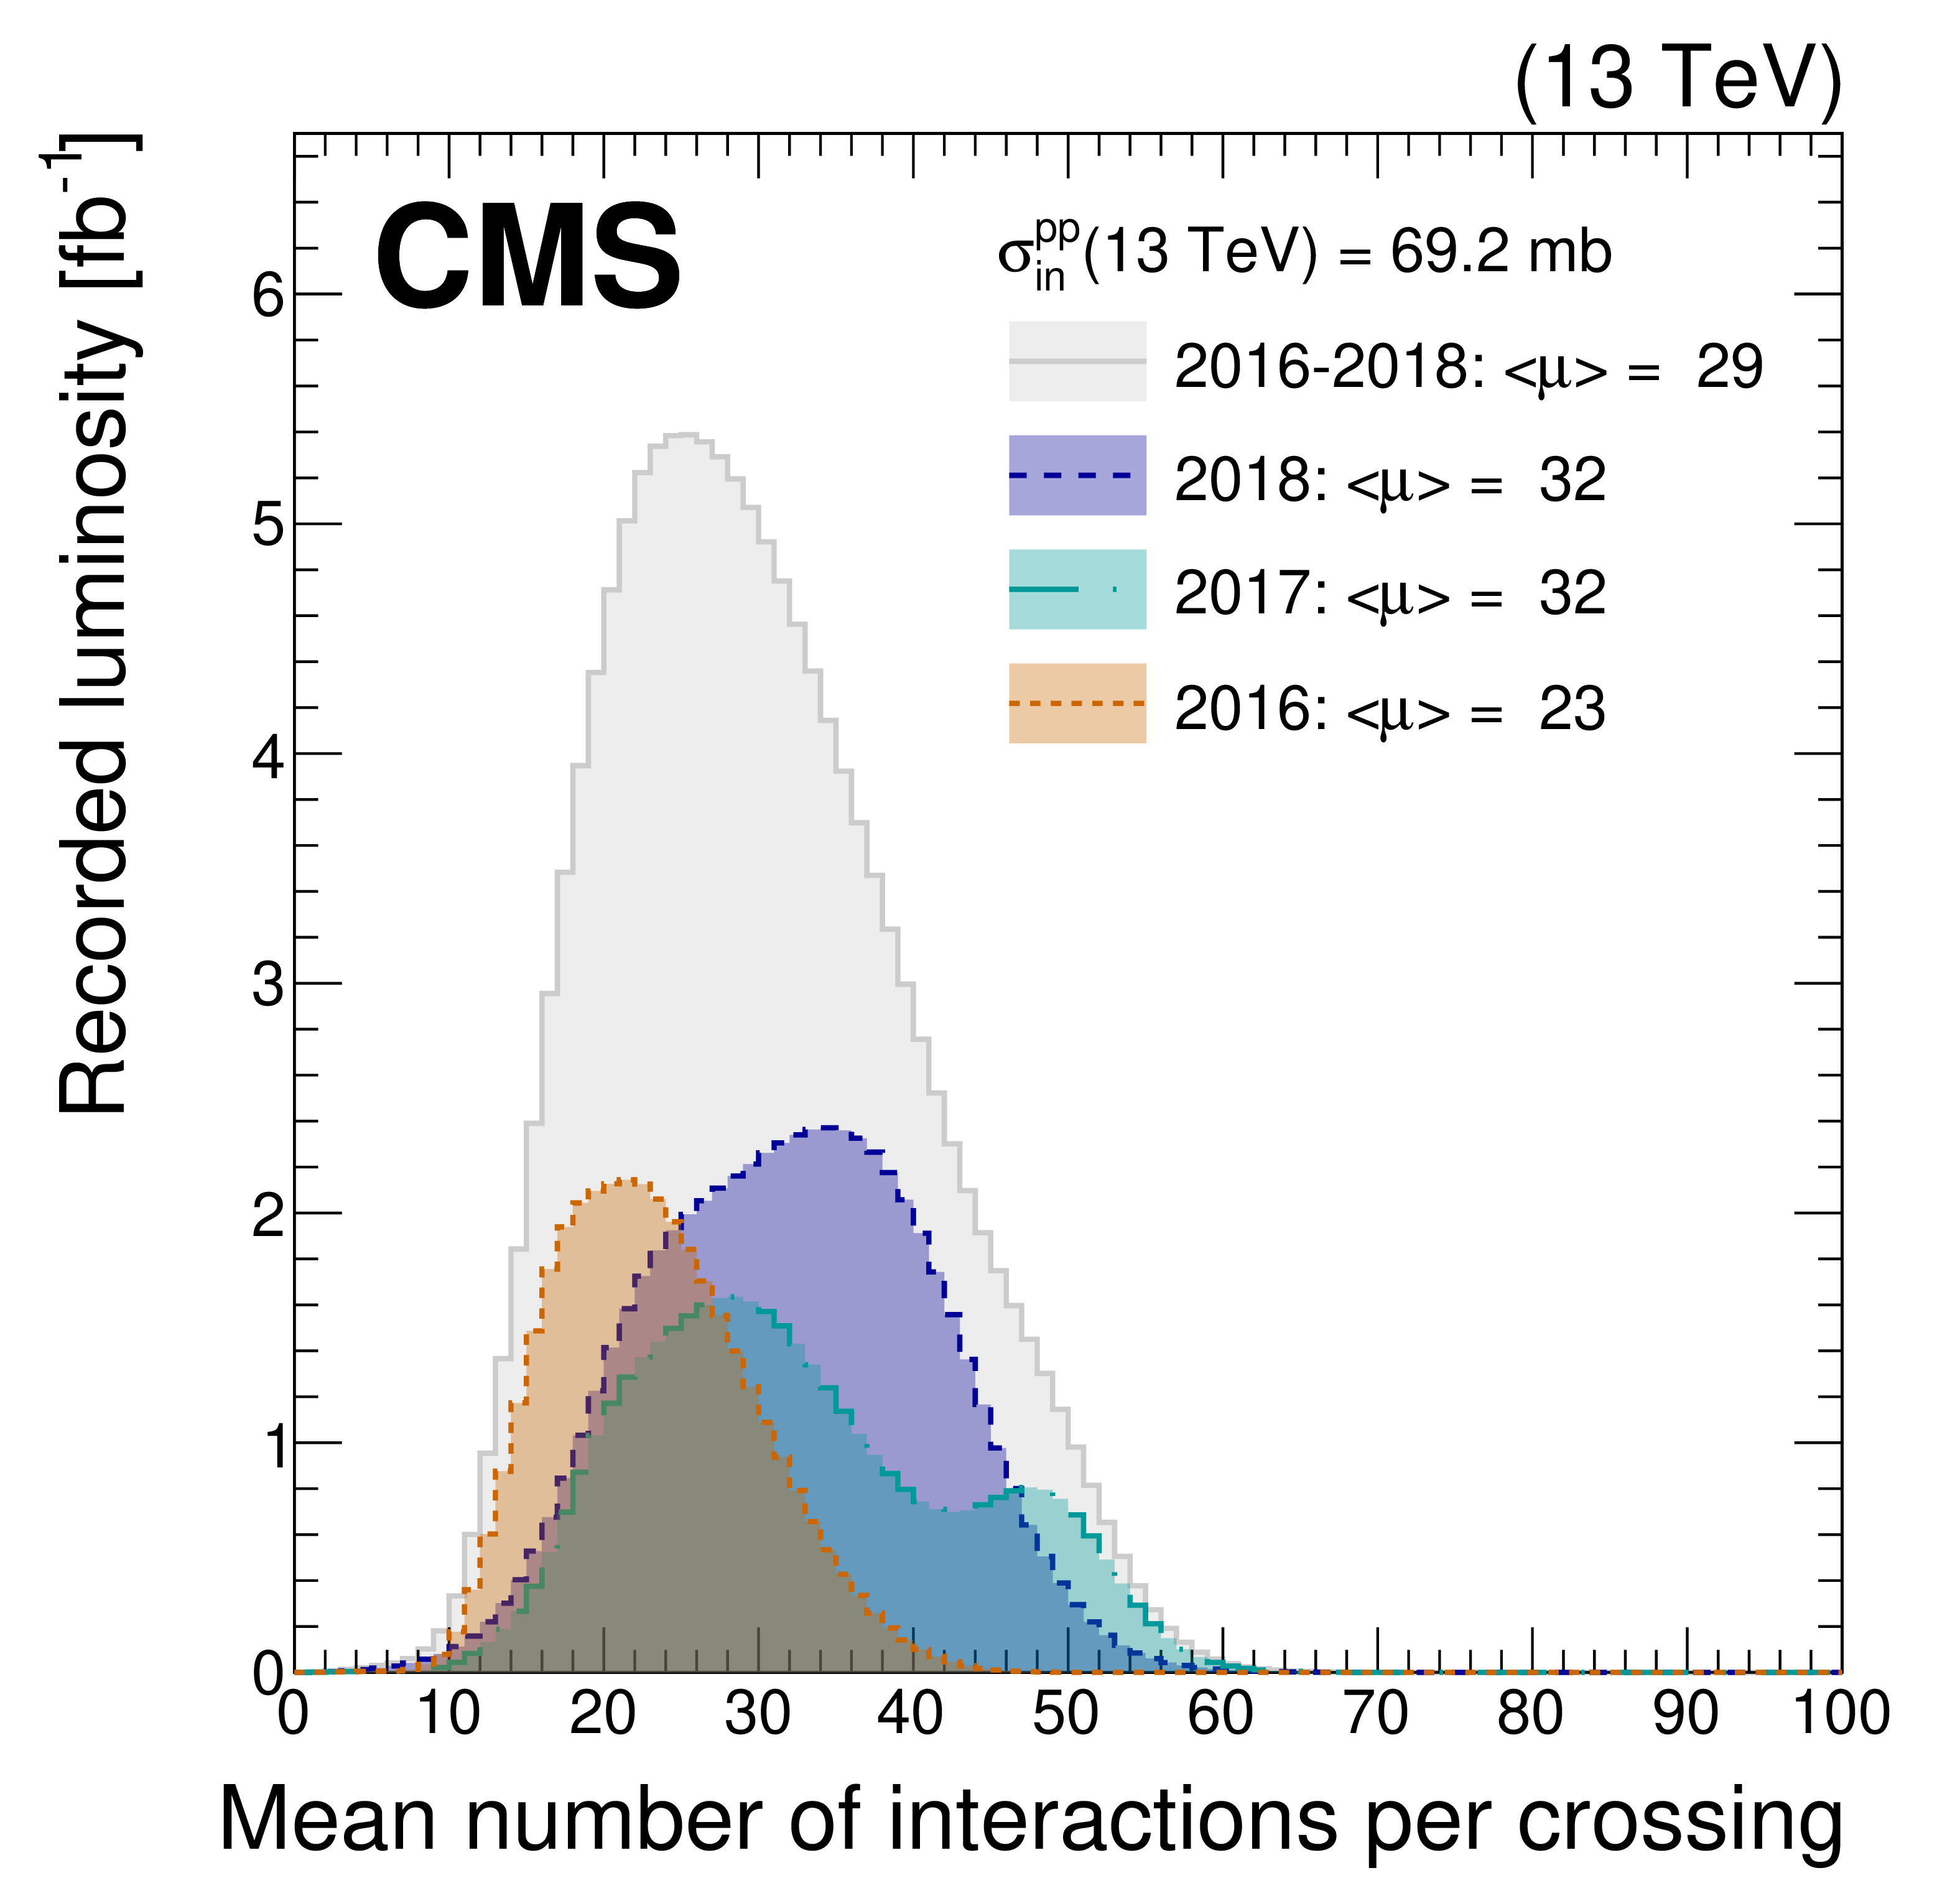
\includegraphics[width=8cm]{figures/ch-2-cern-cms/pileup-run-2-CMS-JME-18-001_Figure_001.png}
    \caption[Distribution of the mean number of inelastic collisions per bunch crossing (pileup) in data, for proton-proton collisions in 2016-2018]{Distribution of the mean number of inelastic collisions per bunch crossing (pileup) in data~\cite{CMS-JME-18-001}, for proton-proton collisions in 2016 (\textit{dotted orange}), 2017 (\textit{dotted light blue}), 2018 (\textit{dotted dark blue}), and integrated over 2016-2018 (\textit{solid grey}). A cross-section of inelastic proton-proton collisions of 69.2 mbarns is assumed. In the running conditions of the High-Luminosity LHC, pileup will reach unprecedented levels of up to 200 per bunch crossing~\cite{CERN-2020-010-HL-LHC-TDR}.}
    \label{fig:pileup-run-2}
\end{figure}

These multiple collisions will lead to higher occupancies in the detector, and particles originating from the pileup interactions can be confused with those originating from the primary vertex. Thus, higher luminosities create more intense pileup conditions, posing a greater challenge to detector performance and particle reconstruction and identification.


\section{The High-Luminosity LHC}
\label{section:HL-LHC}
The High-Luminosity LHC (HL-LHC) is a major upgrade of the LHC scheduled to take place in the late 2020s, that will increase the instantaneous luminosity by a factor of of five beyond the original design value, and the integrated luminosity by a factor of ten~\cite{CERN-2020-010-HL-LHC-TDR}. This will be accomplished through accelerator technological advances: for instance, reduction of the interaction point $\beta^*$ from 0.55 m down to 0.15 m by installation of new final-focusing magnets, and improvements in the geometric luminosity loss factor $F \approx 1$ through the installation of crab cavities that optimize the orientation of colliding bunches. A further discussion of the HL-LHC upgrades for the CMS detector follows in Chapter \ref{chapter:ch-3:phase-2-upgrade-cms}.

\section{The CMS Detector}
\label{section:cms-detector}
We give a brief overview of the Compact Muon Solenoid (CMS) experiment here and discuss each of the subdetectors in more detail in the following sections. The CMS experiment was conceived to study proton-proton and lead-lead collisions at a center-of-mass energy of 14\TeV (5.5\TeV nucleon-nucleon) and at luminosities up to $10^{34}$\percms ($10^{27}$\percms)~\cite{CMS-2008-JINST-3-S08004}~\cite{CERN-EP-2017-110}. Starting from the beam interaction region at the center of the CMS detector, particles first pass through a silicon pixel and strip tracker, in which charged-particle trajectories (tracks) and origins (vertices) are reconstructed from signals (hits) in the sensitive layers. The tracker, electromagnetic calorimeter (ECAL), and hadronic calorimeter (HCAL) are immersed in a high-magnetic-field superconducting solenoid that bends the trajectories of charged particles. After passing through the tracker, electrons and photons are then absorbed in the electromagnetic calorimeter (ECAL) comprised of lead-tungstate scintillating-crystals. The corresponding electromagnetic showers are detected as clusters of energy recording in neighboring cells, from which the direction and energy of the particles can be determined. Charged and neutral hadrons may initiate a hadronic shower in the ECAL as well, which is then fully absorbed in the hadron calorimeter (HCAL). The resulting clusters are used to estimate their direction and energies. Muons and neutrinos pass through the calorimeters with little to no interactions. Neutrinos escaped undetected; muons produce hits in additional gas-ionization chamber muon detectors housed in the iron yoke of the flux-return. A sketch of example particle interactions in a transverse slice of the CMS detector is shown in Fig. \ref{fig:sketch-cms-particle-interactions}. The collision data is recorded with the use of the Level-1 (L1) trigger (discussed in greater detail in \ref{section:phase-1-l1-trigger}), the High-Level Trigger (HLT), and data acquisition systems ensuring high efficiency in selecting physics events of interest. 

\begin{figure}[ht]
    \centering
    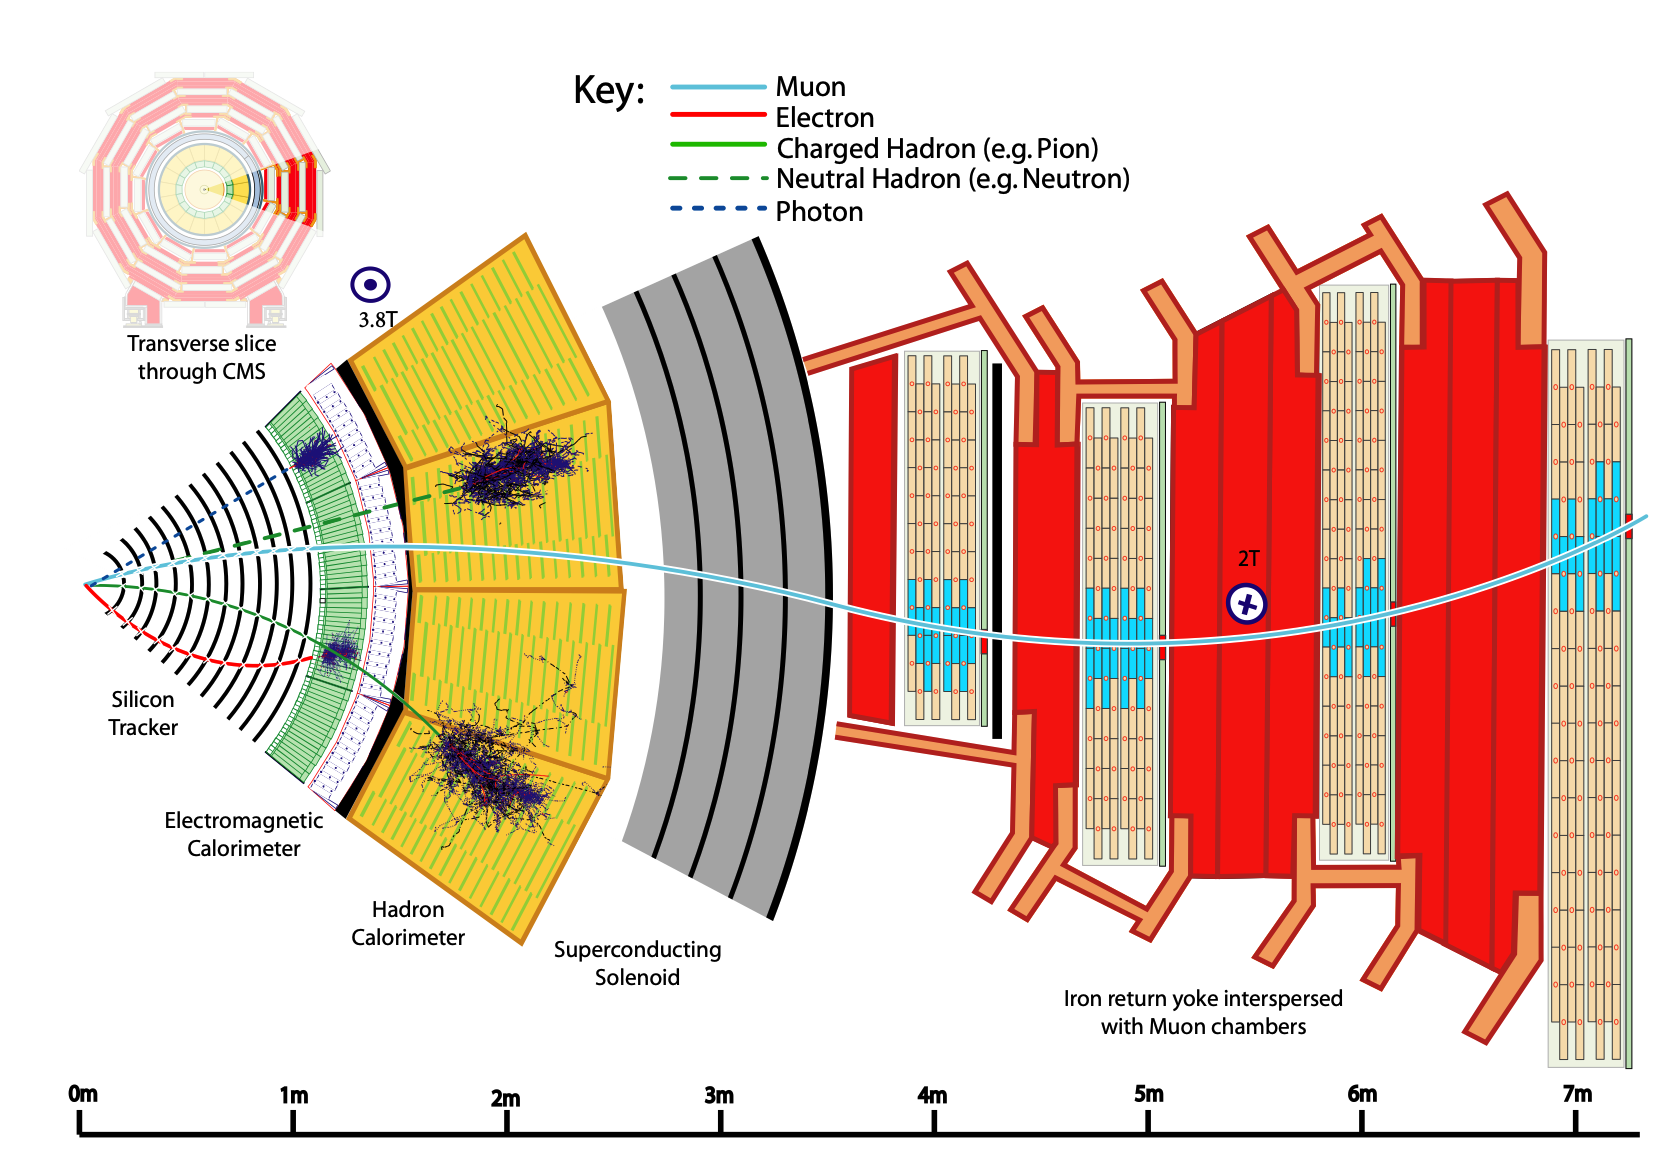
\includegraphics[width=11cm]{figures/ch-2-cern-cms/sketch-cms-particle-interactions.png}
    \caption[Sketch of particle trajectories of muons, electrons, charged and neutral hadrons, and photons in a transverse cross-section of the CMS detector.]{Sketch of particle trajectories of muons, electrons, charged and neutral hadrons, and photons in a transverse cross-section of the CMS detector~\cite{CERN-EP-2017-110}.}
    \label{fig:sketch-cms-particle-interactions}
\end{figure}

CMS uses a right-handed coordinate system~\cite{CMS-2008-JINST-3-S08004}. The origin is centered at the nominal collision point inside the experiment. The $x$ axis points towards the center of the LHC, and the $y$ axis points vertically upwards. The $z$ axis points along the beam direction. The azimuthal angle, $\phi$, is measured from the $x$ axis in the $x$-$y$ plane, and the radial coordinate in this plane is denoted by $r$. The polar angle, $\theta$, is measured from the $z$ axis. The pseudorapidity, $\eta$, is defined as $\eta = -\ln \tan(\theta/2)$. The momentum and energy transverse to the beam direction, denoted by $p_{T}$ and $E_{T}$ respectively, are computed from the $x$ and $y$ components. The momentum imbalance in the transverse plane is called the missing transverse momentum, and its magnitude is denoted by $E_{T}^{\text{miss}}$.

\section{Sub-detectors of CMS}
This section details the sub-detectors of CMS that operate to identify and precisely measure muons, electrons, photons, and jets over a large energy range. 

\subsection{Inner tracking system}

The CMS Tracker performs robust tracking and detailed vertex reconstruction in the 4 T magnetic field of the superconducting solenoidal magnet. The primary sensors used in the tracker are $p^+$ on $n$-bulk devices, which allow high voltage operation and are radiation-resistant~\cite{CERN-LHCC-98-006}~\cite{CERN-LHCC-2017-009-tracker-phase2-tdr}. The active envelope of the CMS Tracker extends to a radius of 115 cm, over a length of approximately 270 cm on each side of the interaction point~\cite{CERN-LHCC-98-006}.
Charged particles in the region $|\eta| \lesssim 1.6$ benefit from the full momentum measurement precision. In this region, a charged particle with $p_T$ of 1000\GeV has a sagitta of $\sim 195$ $\mu$m. The Tracker acceptance extends further to $|\eta| = 2.5$, with a reduced radius of approximately 50 cm.

The high magnetic field of CMS causes low $p_{T}$ charged particles to travel in helical trajectories with small radii. The majority of events contain particles with a steeply falling $p_{T}$ spectrum, resulting in a track density which rapidly decreases at higher radii. 

A schematic view of the current Phase-1 CMS tracker~\cite{CMS-TDR-011-pixel}, including the pixel detector, is shown in Fig. \ref{fig:phase-1-tdr-tracker-schematic}. The Phase-1 pixel detector consists of three barrel layers (BPIX) at radii of 4.4 cm, 7.3 cm, and 10.2 cm, and two forward/backward disks (FPIX) at longitudinal positions of $\pm$ 34.5 cm and $\pm$ 46.5 cm, and extending in radius from about 6 cm to 15 cm. These pixelated detectors produce 3D measurements along the paths of charged particles with single hit resolutions between 10-20 $\mu$m. 


\begin{figure}[ht]
    \centering
    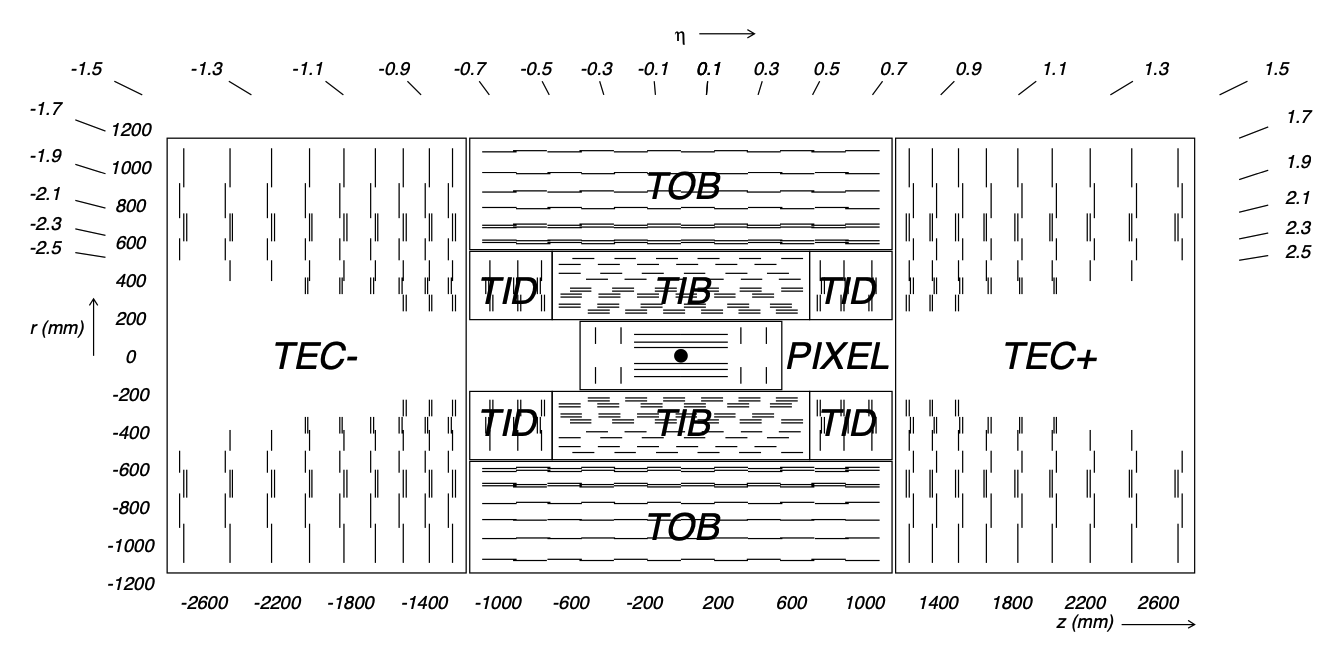
\includegraphics[width=11cm]{figures/ch-2-cern-cms/phase-1-tdr-tracker-schematic.png}
    \caption[Cross section of the current Phase-1 CMS tracker.]{Cross section of the current Phase-1 CMS tracker~\cite{CMS-TDR-011-pixel}. Each line represents a detector module. Double lines indicate back-to-back modules which deliver two-dimensional (stereo) hits in the strip tracker.}
    \label{fig:phase-1-tdr-tracker-schematic}
\end{figure}

After the pixel and on their way out of the tracker, particles pass through the silicon strip tracker which reaches out to a radius of 130 cm (Fig. \ref{fig:phase-1-tdr-tracker-schematic}). The sensor elements in the strip tracker are single-sided $p$-on-$n$ type silicon micro-strip sensors~\cite{CMS-2008-JINST-3-S08004}. The silicon strip detector consists of four inner barrel (TIB) layers assembled in shells, with two inner endcaps (TID), each composed of three small discs. The outer barrel (TOB) consists of six concentric layers. Two endcaps (TEC) close off the tracker on either end. 


\subsection{ECAL} 
The electromagnetic calorimeter (ECAL) of CMS measures electromagnetic energy deposits with high granularity. One of the driving criteria in the design was the capability of detecting the Standard Model Higgs boson decay to two photons (in fact, the channel in which the 125\GeV Higgs boson was discovered at CMS). 
ECAL is a hermetic homogeneous calorimeter comprised of 61,200 lead tungstate (PbWO$_4$) crystals mounted in the central barrel, with 7,324 crystals in each of the two endcaps~\cite{CMS-2008-JINST-3-S08004}. A preshower detector is located in front of the endcap crystals. Avalanche photodiodes (APDs) are used as photodetectors in the barrel and vacuum phototriodes (VPTs) in the endcaps. 

The design of the ECAL is driven by the behaviour of high-energy electrons, which predominantly lose energy in matter via bremsstrahlung, and high-energy photons by $e^+ e^-$ pair production. The characteristic amount of matter traversed for these interactions is the radiation length $X^0$, usually measured in units of g cm$^-2$. The radiation length is also the mean distance over which a high-energy electron loses all but $1/e$ of its energy via bremsstrahlung~\cite{workman_review_2022}. Thus high granularity in $\eta$ and $\phi$, and the length of the ECAL crystals, is designed to capture the shower of $e/\gamma$ produced by electrons and photons.

The barrel part of the ECAL (EB) covers the pseudorapidity range $|\eta| < 1.479$~\cite{CMS-2008-JINST-3-S08004}. The barrel granularity is 360-fold in $\phi$ and ($2 \times 85$)-fold in $\eta$. The crystal cross-section corresponds to approximately $0.0174 \times 0.0174$ in $\eta-\phi$ or $22 \times 22$ mm$^2$ at the front face of the crystal, and $26 \times 26$ mm$^2$ at the rear face. The crystal length is 230 mm, corresponding to 25.8 $X_0$.

The ECAL read-out acquires the signals of the photodetectors~\cite{CMS-2008-JINST-3-S08004}. At each bunch crossing, digital sums representing the energy deposit in a trigger tower, comprising $5 \times 5$ crystals in $\eta \times \phi$, are generated and sent to the Level-1 trigger system (detailed in Section \ref{section:phase-1-l1-trigger}).

\subsection{HCAL}
The hadronic calorimeter (HCAL) of CMS measures hadronic energy, which is key to characterizing the presence of apparent missing transverse energy which could arise from hadron jets and neutrinos or exotic particles~\cite{CMS-2008-JINST-3-S08004}. A schematic of the components of HCAL are shown in Fig. \ref{fig:phase-1-HCAL-schematic}. The HCAL barrel (HB) and endcaps (HE) are located outside of the tracker and the ECAL, spanning a radius of 1.77 m (outer extent of ECAL) up to 2.95 m (inner extent of the magnet coil). An outer hadron calorimeter (HO) is placed outside the solenoid to complement the barrel calorimeter. Beyond $|\eta| = 3$, the forward hadron calorimeter (HF) at 11.2 m from the interaction point extend the pseudorapidity coverage to $|\eta| = 5.2$.

\begin{figure}[ht]
    \centering
    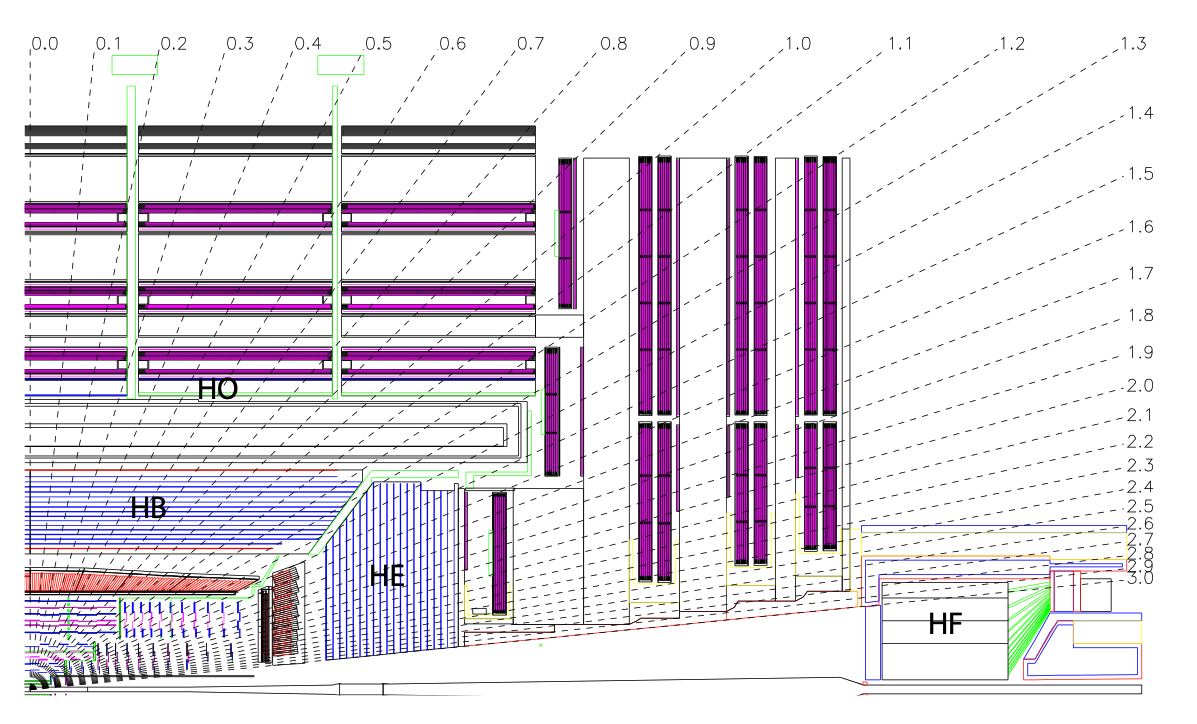
\includegraphics[width=11cm]{figures/ch-2-cern-cms/phase-1-HCAL-schematic.png}
    \caption[Longitudinal view of the CMS detector showing the hadron calorimeter barrel (HB), endcap (HE), outer (HO), and forward (HF) calorimeters.]{Longitudinal view of the CMS detector showing the hadron calorimeter barrel (HB), endcap (HE), outer (HO), and forward (HF) calorimeters from~\cite{CMS-2008-JINST-3-S08004}.}
    \label{fig:phase-1-HCAL-schematic}
\end{figure}

The HB is a sampling calorimeter covering the pseudorapidity range $|\eta| < 1.3$~\cite{CMS-2008-JINST-3-S08004}. It consists of 36 identical azimuthal wedges which form two half-barrels (HB+ and HB-), with a segmentation of $(\Delta \eta, \Delta \phi) = (0.087, 0.087)$. The HE covers pseudorapidity $1.3 < |\eta| < 3$. The HB and endcap HE calorimeters are sampling calorimeters which use brass as the absorber and plastic scintillator as the active material. Light from the plastic scintillator is wavelength-shifted and captured in optic fibers which are read out by front-end electronics~\cite{CMS-TDR-010-2012}. 

In the central pseudorapidity region, the combined stopping power of EB plus the HB is insufficient to contain hadron showers~\cite{CMS-2008-JINST-3-S08004}. To ensure adequate sampling depth, the hadron calorimeter is extended with a tail catcher, the HO. The size and position of the tiles are designed to roughly map the layers of the HB to make towers with the same granularity of $0.087 \times 0.087$ in $\eta$ and $\phi$. HO uses the same active material as the HB and HE calorimeters, but uses the steel return yoke and magnet material of CMS as absorbers~\cite{CMS-TDR-010-2012}. 


The HF is a Cherenkov calorimeter based on a steel absorber and quartz fibers which run longitudinally through the absorber and collect Cherenkov light, primarily from the electromagnetic component of showers developed in the calorimeter~\cite{CMS-TDR-010-2012}. Photomultiplier tubes are used to  collect light from the quartz fibers. The HF is designed to survive in the harsh radiation conditions and high particle flux of the forward region. On average, 760\GeV per proton-proton interaction is deposited into the two forward calorimeters, compared to only 100\GeV for the rest of the detector~\cite{CMS-2008-JINST-3-S08004}. Furthermore, this energy has a pronounced maximum at the highest rapidities.

\subsection{Muon detectors}
The CMS muon system is designed to have the capability of reconstructing the momentum and charge of muons over the kinematic range of the LHC, since muons are a powerful handle on signatures of interesting processes over the high background rate of the LHC~\cite{CMS-2008-JINST-3-S08004}. For instance, the decay of the Standard Model Higgs boson into $ZZ$, which in turn decay to 4 leptons, can be reconstructed with high 4-particle mass resolution if all the leptons are muons, since muons are less affected than electrons by radiative losses in the tracker material. 

The muon system consists of a cylindrical barrel section and two planar endcap regions~\cite{CMS-2008-JINST-3-S08004}. The barrel muon detector consists of drift tube (DT) chambers covering the pseudorapidity region $|\eta| < 1.2$ (Fig. \ref{fig:phase-1-muon-barrel-DT-schematic}). The DTs can be used as tracking detectors due to the barrel region's characteristic low neutron-induced backgrounds, low muon rate, and relatively uniform 4T magnetic field contained in the steel yoke. 

\begin{figure}[ht]
    \centering
    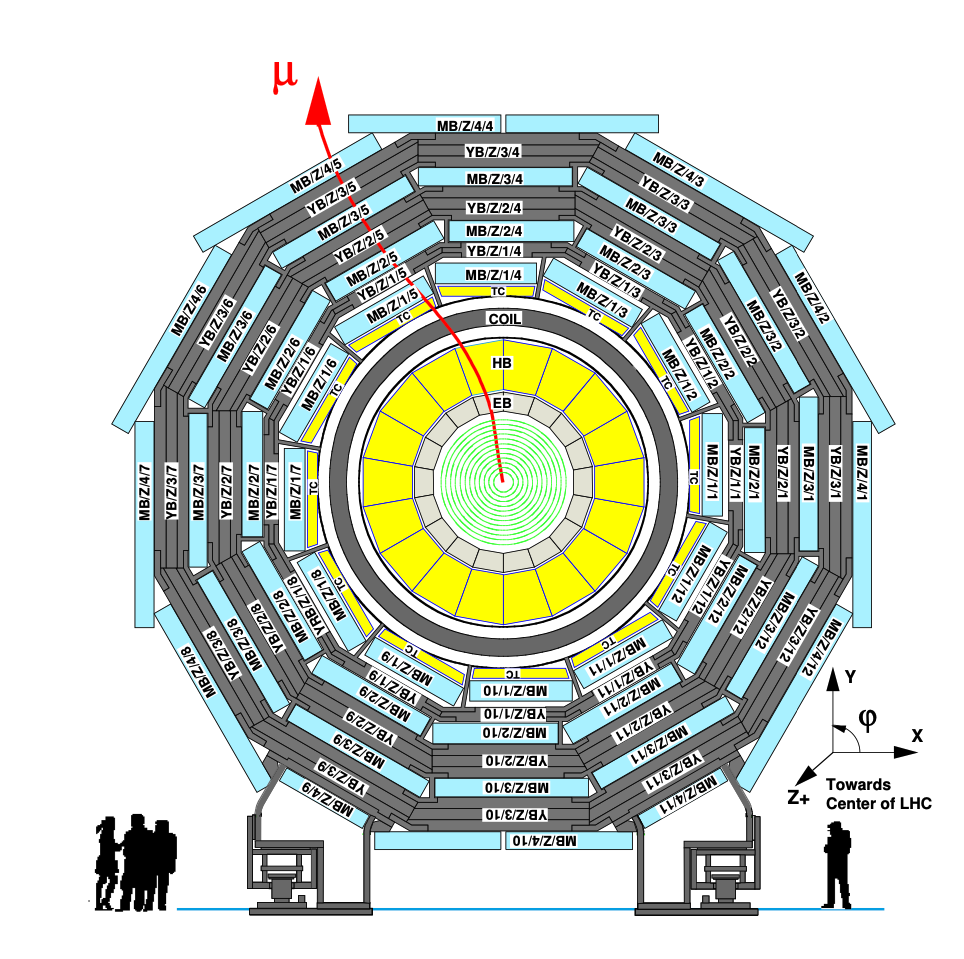
\includegraphics[width=11cm]{figures/ch-2-cern-cms/phase-1-muon-barrel-DT-schematic.png}
    \caption[Layout of the CMS barrel muon drift tube (DT) chambers in one of the five wheels.]{Layout of the CMS barrel muon drift tube (DT) chambers in one of the five wheels from~\cite{CMS-2008-JINST-3-S08004}. The DTs are organized in 12 sectors of the yoke barrel (YB). In each of the 12 sectors of the yoke, there are 4 muon chambers per wheel (MB1, MB2, MB3, and MB4).}
    \label{fig:phase-1-muon-barrel-DT-schematic}
\end{figure}

In the two endcap regions, the muon rates and background levels are high and the magnetic field is large and non-uniform~\cite{CMS-2008-JINST-3-S08004}. Here, the muon system uses cathode strip chambers (CSCs) to identify muons between $0.9 < |\eta| < 2.4$. The cathode strips of each chamber run radially outwards and provide a precision measurement in the $r-\phi$ bending plane. The anode wires run approximately perpendicular to the strips and are read out in order to measure $\eta$ and the beam-crossing time of a muon. 

% 2008 JINST 3 S08004, page 164
In addition to the DT and CSC, a dedicated trigger system consisting of resistive plate chambers (RPCs) in the barrel and endcap regions provide a fast, independent, and highly-segmented trigger with a sharp $p_T$ threshold over a large portion of the pseudorapidity range ($|\eta| < 1.6$) of the muon system~\cite{CMS-2008-JINST-3-S08004}. RPCs have good time resolution but coarser position resolution compared to the DTs or CSCs. The RPCs also play a role in resolving ambiguities in reconstructing tracks from multiple hits in a chamber. 

\subsection{The Level-1 Trigger}
\label{section:phase-1-l1-trigger}
The design performance of the LHC corresponds to an instantaneous luminosity of $10^{34}$ cm$^{-2}$ s$^{-1}$ with a 25 ns bunch crossing rate, giving an average pile-up (number of simultaneous events) of 25 per bunch crossing~\cite{CMS-TDR-012}. The large number of minimum bias events per bunch crossing, combined with the small cross-sections of possible physics discovery signatures, necessitates a sophisticated event selection system for filtering this large event rate, as it is impossible to save all events. This data filtering system is implemented by CMS in two stages. The first stage is the Level-1 (L1) Trigger, which is deployed in custom electronic hardware systems and is responsible for reducing the event rate to around 100 kHz. The second stage is the High-Level Trigger (HLT) which is described in Section \ref{section:phase-1-high-level-trigger}. This section describes the Phase-1 configuration of the Level-1 Trigger.


The L1 Trigger data flow of Phase-1 is shown in Fig. \ref{fig:phase-1-level-1-trigger-dataflow}~\cite{CMS-TDR-012}, with organization into the L1 calorimeter trigger, the L1 muon trigger, and the L1 global trigger. 

\begin{figure}[ht]
    \centering
    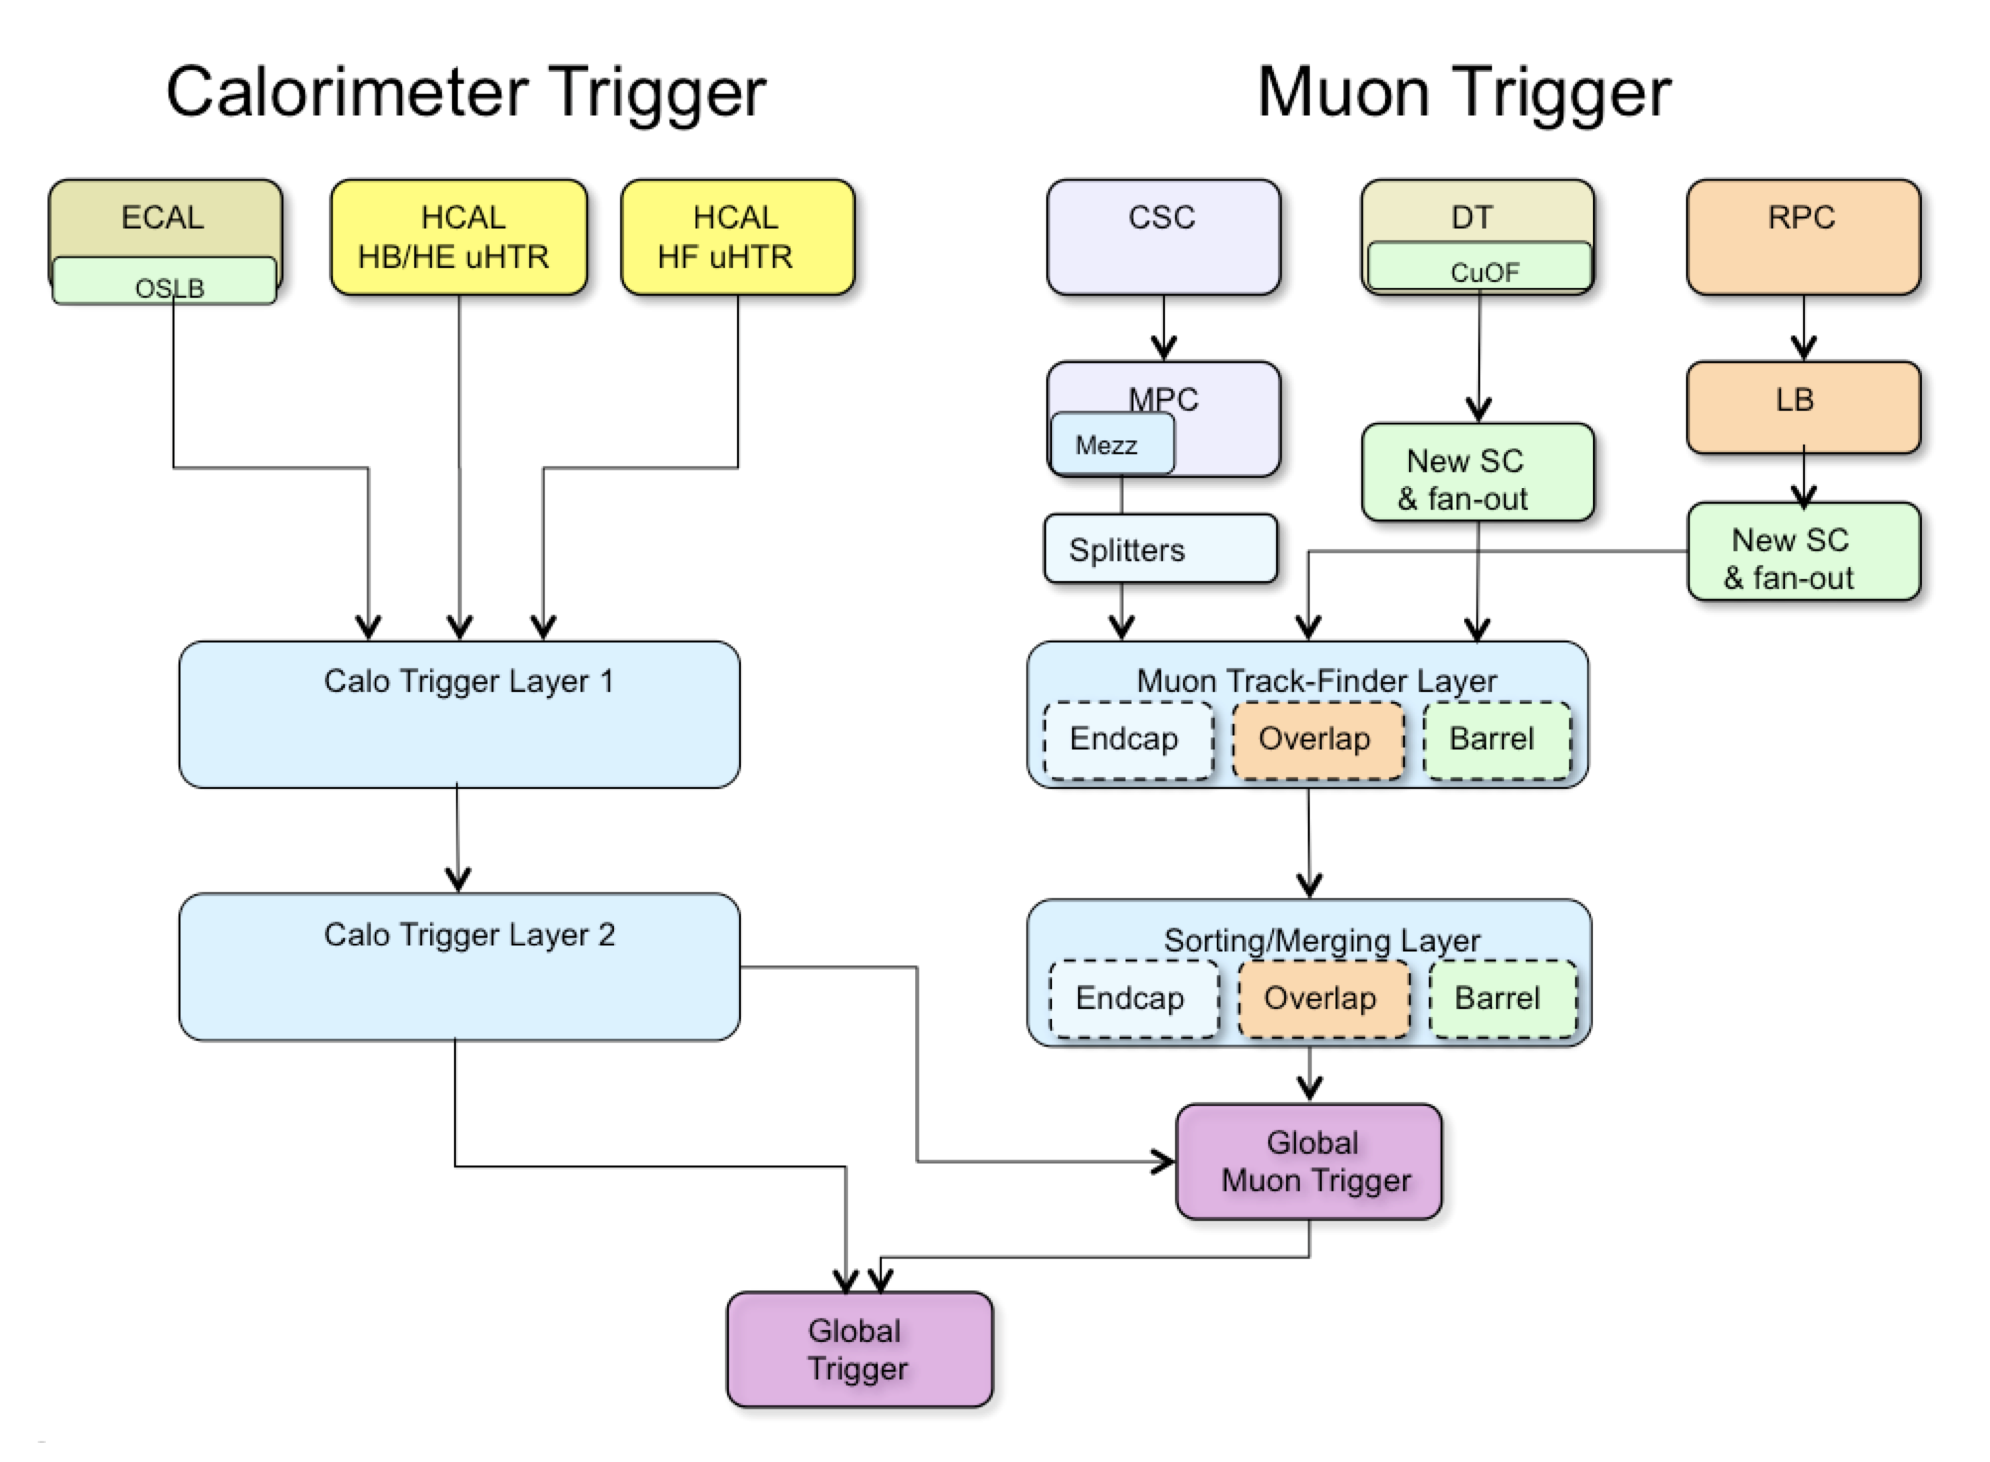
\includegraphics[width=11cm]{figures/ch-2-cern-cms/phase-1-level-1-trigger-dataflow.png}
    \caption[Dataflow for the Phase-1 Level-1 Trigger.]{Dataflow for the Phase-1 Level-1 Trigger~\cite{CMS-TDR-012}, which is implemented in custom hardware and is responsible for reducing the event rate from the LHC bunch crossing frequency of 400 MHz (bunch crossings every 25 ns) to a maximum rate of 100 kHz. In Phase-1, the Level-1 Trigger has access to information from the calorimeter and muon detectors.}
    \label{fig:phase-1-level-1-trigger-dataflow}
\end{figure}

The L1 calorimeter trigger begins with trigger tower energy sums formed by the ECAL, HCAL, and HF Trigger Primitive Generator (TPG) circuits from the individual calorimeter cell energies. In the original configuration, the ECAL energies were accompanied by a bit indicating the transverse extent of the electromagnetic energy deposits, and the HCAL energies were accompanied by a bit indicating the presence of minimum ionizing energy~\cite{CERN-LHCC-2000-038}. Between Long Shutdowns 1 and 2 (LS1 and LS2), HF was upgraded to provide finer granularity information to the trigger, and the HCAL barrel and endcap front-end electronics were upgraded to provide high-precision timing information and depth segmentation information. 

In the original design of the L1 calorimeter trigger, the trigger primitives are processed by the Regional Calorimeter Trigger (RCT, upgraded to Calo Layer 1 after LS2) which finds isolated and non-isolated electron/photon candidates~\cite{CMS-TDR-012}. At this stage, electrons/photons candidates are treated together since they cannot be definitively distinguished at this stage due to lack of tracking information in the L1 trigger. The Global Calorimeter Trigger (GCT, upgraded to Calo Layer 2 after LS2) sorts further the candidate electrons/photons, finds jets (classified as central, forward, and tau) using the $E_T$ sums and performs calibration of the clustered jet energies, and calculates global quantities such as missing $E_T$. It sends the top four candidates of each type to the global trigger (GT)~\cite{CMS-TDR-012}.

Each of the L1 muon triggers has its own trigger logic~\cite{CERN-LHCC-2000-038}. The RPC strips are connected to a Pattern Comparator Trigger (PACT), which forms trigger segments that are used to build tracks and calculate $p_{T}$. The RPC logic also provides some hit data to the CSC trigger system to resolve ambiguities caused by two muons in the same CSC. The CSCs form local charged tracks (LCTs) from the cathode strips, which are combined with the anode wire information. LCTs are combined into full muon tracks and assigned $p_{T}$ values. 

The Global Muon Trigger (GMT) sorts the RPC, DT, and CSC muon tracks, converts these tracks to the same $\eta$, $\phi$, and $p_{T}$ scale, and validates the muon sign~\cite{CERN-LHCC-2000-038}. It improves the trigger efficiency by merging muon candidates that were detected in two complementary sub-systems (i.e. DT+RPC, or CSC+RPC). The GMT also contains logic to correlate the found muon tracks with an $\eta-\phi$ grid of quiet calorimeter towers to determine if the muons are isolated, as well as logic to remove duplicate candidates originating in the overlap regions from both DT and CSC systems. The final collection of muons are sorted based on their initial quality, correlation, and $p_{T}$, and the top four muons are sent to the Global Trigger~\cite{CERN-LHCC-2000-038}. 

Information from the GCT and GT are sent to the Global Trigger (GT), which makes the Level-1 Accept (L1A) decision to either discard or accept the bunch crossing~\cite{CERN-LHCC-2000-038}. This is accomplished by sorting ranked trigger objects that are accompanied by positional information in $\eta$ and $\phi$, permitting the trigger to applying criteria with thresholds that can vary based on the location of the trigger objects, and/or to require trigger objects to be close to or opposite from each other. The GT L1A decision arrives at the detector front end with a 3.8 $\mu$s latency after the interaction at a rate which is required to be less than 100 kHz, and triggers a full readout of the detector for further processing.



\subsection{The High-Level Trigger}
\label{section:phase-1-high-level-trigger}
The HLT is implemented in software running on a large computer farm of fast commercial processors~\cite{CMS-TDR-022-HLT}~\cite{Foudas:2008dt}. The algorithms in HLT have access to full data from all CMS sub-detectors, including the tracker, with full granularity and resolution. The HLT reconstruction software is similar to what is used offline for full CMS data analysis. As a result, the HLT can calculate quantities with a resolution comparable to the final detector resolution, compared to the L1 Trigger. The HLT performs more computationally-intensive algorithms, such as combining tau-jet candidates in the calorimeter with high-$p_T$ stubs in the tracker, to form a hadronic tau trigger. The maximum HLT input rate from the L1 Trigger is 100 kHz, and the HLT output rate is approximately 100 Hz. 

The HLT contains trigger paths, each corresponding to a dedicated trigger~\cite{twiki_SoftwareGuide_HLT}.  A path consists of several steps implemented as software modules. Each HLT trigger path must be seeded by one or more L1 trigger bits: the first module always looks for a L1 seed, consisting of L1 bit(s) and L1 object(s). Each module performs a well-defined task such as unpacking (raw to digitized quantities), reconstruction of physics objects (electrons, muons, jet, missing transverse energy, etc.), making intermediate decisions that trigger more detailed reconstruction modules, and calculating the final decision for the trigger path. If an intermediate filter decision is negative, the rest of the path is not executed, and the trigger rejects the event.


\subsection{Particle reconstruction}
To build a description of the physics objects present in the particle collision, the basic elements from the detector layers (tracks and clusters of energy) are correlated to identify each particle in the final state. Measurements from different sub-detectors are combined to reconstruct the particle properties. This approach is called particle-flow (PF) reconstruction~\cite{CERN-EP-2017-110}. Key to the success of the PF reconstruction is the fine spatial granularity of the detector layers. Coarse-grained detectors can cause the signals from different particles to merge, especially within jets. However, if the subdetectors are sufficiently segmented to separate individual particles, it becomes possible to produce a global event description that identifies all physics objects with high efficiencies and resolution.

\subsection{Data storage and computational infrastructure}

The LHC generates over 15 petabytes (15 million gigabytes) of data every year, necessitating a flexible computing system that can be accessed by researchers working at the four main LHC experiments: ALICE, ATLAS, CMS, and LHCb. The Worldwide LHC Computing Grid (WLCG)~\cite{computing-Worldwide:1997398} is a global collaboration of computer centers that links thousands of computers and storage systems in over 170 centers across 41 countries. These centers are arranged in ``tiers'', and provide near real-time access to users processing, analyzing, and storing LHC data. One of the final stages of data analysis at LHC experiments is large-scale data processing taking place over distributing computing, for instance, with the use of Condor~\cite{condor-article}, a distributed, scalable, flexible batch processing system which accepts a computing job, allocates a resource to it, executes it, and returns the result back to a user transparently. 
 
